\section{Markt}
\subsection{Einleitung}
Im folgenden Kapitel soll ein grober Überblick und eine Einleitung zum IT-Consulting Markt gegeben werden. 
Ziel einer solchen Recherche ist zum einen Informationen zu sammeln, die strategische Möglichkeiten für Expansion, Kooperation oder Offshoring aufzeigen, 
als auch die Wettbewerbssituation besser einzuschätzen, um daraus Handlungsalternativen abzuleiten. 
In zahlreichen Studien tauchen in diesem Zusammenhang häufig sehr weitgefasste Begriffe auf wie „technology industry“ oder "IT-service-market" auf. 
Die Grenzen der Bandbreite der darin enthaltenen Beratungsleistungen ist in diesem Zusammenhang unscharf. Eine Differenzierung ist aufgrund der Komplexität der Zusammensetzung des Dienstleistungsspektrums daher nur in groben Umfang möglich.
Als Maßzahl wird in Studien ein grober Anteil von mind. 40\% für ausschließlich beratende Tätigkeiten berücksichtigt, um in eine IT-Consulting äquivalente Kategorie zu fallen.
Es gibt zahlreiche Schlüsselfaktoren die für die Einschätzung des Marktes in den jeweiligen Ländern bzw. Kontinenten aufschlussreich sind. 
Allerdings ist eine Erhebung sehr zeitaufwändig oder/und teuer. Es gibt zahlreiche Marktstudien von großen Marktforschungsunternehmen, wie z.B. Gartner, die man ab ca. 1000€  erwerben kann, die aber nur Teilaspekte abdecken. 
Die Tatsache, dass es kaum kostenfreie umfassendere Studien dazu gibt, dafür aber zahlreiche kostenpflichtige Studien zu hohen Preisen, lässt vermuten, dass es zumindest aufgrund des niedrigen Angebots eine moderate Nachfrage nach Marktinformationen im Bereich IT-Consulting gibt.
 Es wird sich hier daher auf eine Vielzahl von Studien bezogen, welche teilweise aus verschiedenen Jahren stammen, aber dennoch verhältnismäßig neu sind.
 Ziel ist es sich dem Thema anzunähern und die Schlüsselfaktoren zu überlegen und deren konkreten Größen zu ermitteln.

\subsection{Teilaspekte}
Nachfolgend soll daher zuerst einmal begründet werden, welche Teilaspekte für eine Marktrecherche im IT-Consulting für eine Studie als besonders relevant erachtet werden.
Ein Großteil der Arbeit liegt in der Konzeption einer solchen Recherche. Da dies aufgrund der hohen Komplexität der Märkte keine allzu klare Sache ist. Eindeutige Prognosen können daraus folglich nicht resultieren, jedoch lassen sich auf Basis diverser Daten vernünftige Annahmen anstellen, die es wiederum zu verifizieren gilt. 
\subsubsection{Gewinn- und Umsatzzahlen von Großunternehmen weltweit/Länder spezifisch}
Diese Daten sind gut zugänglich und liefern eine grobe Richtzahl über Umsatz und Erfolg in der Branche. 
Außerdem spiegeln die Wachstumsraten und Gewinne von Großunternehmen derzeit auch gut den gesamten Markt wieder. 
Des Weiteren dient es dazu die ermittelten erfolgreichen Unternehmen zu beobachten und deren  Wettbewerbsvorteile zu erkennen, ggbfs. zu adaptieren oder gar zu übertrumpfen.
Außerdem spiegelt es den Erfolg dieser Unternehmen im jeweiligen Land wieder. So kann ein Unternehmen, welches z.B. auf SAP spezialisiert ist, zwar in Brasilien erfolgreich sein, aber in China trotz guter Marktlage nicht. 
 Derartige Diskrepanzen bieten dann wieder Informationen um Vermutungen aufzustellen und diese weiter zu untersuchen (wenig verwendete SAP Software China, starke Konkurrenz etc.) oder um allgemeine Niveauunterschiede zwischen Ländern abzuleiten.

\subsubsection{IT-Consulting Gesamtumsatz und Marktwachstum je Land}
Diese Kennzahlen liefern wichtige Hinweise, wie sich die Branche weiter entwickeln wird und wie sehr sie schon entwickelt ist. 
Diese Daten dienen dazu um Rückschlüsse auf die Nachfrage von IT-Consulting Leistungen zu ziehen. 
Dazu werden natürlich noch eine Reihe weitere Daten benötigt, wie Gesamtmarktvolumen und Gesamtwirtschaftswachstum, um die Kennzahlen ins Verhältnis zu setzen.
 Außerdem muss darauf geachtet werden was die Kennzahlen unter Umständen verfälscht wie z.B. die Ländergröße, wodurch eher ein höherer Umsatz pro Land entsteht. 
 Somit werden unter Umständen wieder weitere Kennzahlen benötigt, um diese Faktoren ordnungsgemäß bewerten zu können.
Der IT-Consulting Umsatz und das Wachstum je Land ist im Verhältnis zu anderen Kenngrößen durchaus in vertretbaren Umfang anhand von öffentlichen Studien erfassbar. 
Daher sollen diese Größen im nächsten Abschnitt einzeln nach Ländern aufgelistet und erläutert werden. 
 Dabei ist zu berücksichtigen, dass auf die daraus resultierenden Anteile und Kennzahlen kein Anspruch auf absolute Korrektheit gelegt werden kann. 
 Hierfür müssten diese Kennziffern noch mehrfach überprüft und eventuelle Verwässerungsfaktoren herausgerechnet werden. 
 Für einen generellen Überblick und eine grobe Quantifizierung sind sie jedoch durchaus brauchbar. So können auf dieser Basis dieser weitere Vermutungen angestellt und entsprechende Recherchen unternommen werden.
Daher wurde sich dazu entschieden diesen Teilaspekt für die Recherche auszuwählen. (siehe  \ref{subsubsec:Gesamtumsatz} \nameref{subsubsec:Gesamtumsatz} auf Seite \pageref{subsubsec:Gesamtumsatz})

 \subsubsection{Firmengrößen im IT-Consulting}
Ein wichtiger Einflussfaktor um die Konkurrenzsituation festzustellen ist die Beschaffenheit des Marktes nach Unternehmensgrößen.
 Es stellt sich die Frage, ob eher Großkonzerne, mittelständische Unternehmen oder gar interne Mitarbeiter für die strategische und ganzheitliche IT beauftragt werden.
 Hier kann die durchschnittliche Firmengröße herangezogen werden um eine Schätzung vorzunehmen. So gibt es Länder die eher einen breiten Mittelstand haben oder eher zu Großkonzernen neigen. 
 Allerdings ist dies nur bedingt auch für das IT-Consulting zutreffend. 
Möglichkeiten zur Ermittlung der Marktbeschaffenheit benötigen daher mindestens einen der folgenden Schritte oder eine Kombination aus diesen:
\begin{itemize}
\item Analyse der Unternehmensgrößen des Landes
\item Berechnung der Marktanteile der größten Unternehmen und Bewertung des Restwertes
\item Statistische Stichproben / Befragungen
\item Beschaffung von Studien oder Beauftragung eines Marktforschungsunternehmen
\end{itemize}
Die resultierenden Informationen zur Beschaffenheit gibt wertvolle Hinweise über das Angebot in der Branche. 
So können von diesem Wissenstandpunkt aus die konkreten Angebote analysiert werden und ggbfs. Chancen abgeleitet werden. 
So können beispielsweise große Unternehmen aufgrund Skalierungseffekten möglicherweise bessere Qualität anbieten als ein breiter Mittelstand, gleichzeitig die Nachfrage nach mittelständischen Unternehmen aufgrund günstigerer Preise attraktiver sein. 
Eine tiefgehende Analyse ist jedoch sehr komplex und würde Stoff für eine eigenständige Studie liefern. Daher soll hier auf den Bedarf hingewiesen werden.


 \subsubsection{Politik / Rechtslage}
Die politische und rechtliche Lage ist ein wichtiger Faktor für die Wahl eines Standortes oder die Zusammenarbeit mit einem Land. Gleichzeitig ist es ein Faktor der die Entwicklung der Branche beeinflusst.
Besonderen Einfluss haben die folgenden Faktoren auf die IT-Consulting Branche:
\begin{itemize} 
\item {generelle staatliche Subventionen / Investitionen in die IT}

 Staatliche Förderprogramme und Subventionen stellen eine wichtige Finanzierungsmethode für Entwicklungsprojekte oder Existenz bedrohte Unternehmen dar. Diese sind entweder zinsgünstige Darlehen oder gar nicht zurückzuzahlen.
 Solche finanziellen Unterstützungen treiben natürlich die Forschung und den allgemeinen Wissenstransfer voran. Insbesondere das IT-Consulting ist eine reine Wissensbranche. Profitiert also die Entwicklung, profitiert auch das IT-Consulting von den neuen Erkenntnissen. 
 Umso wichtiger sind folgrich auch Bildungsinvestitionen und Subventionen. Folglich kann es als Anreiz zur Gründung von Startups und damit die Innovativität der IT-Landschaft fördern. Neue Technologien und Erkenntnisse führen zu neuen Handlungsalternativen. Dies erhöht die Komplexität von Entscheidungsprozessen und Nachfrage nach Beratungsleistungen.
Ein Wissen über Staatssubventionen kann daher hilfreich sein, um das Entwicklungspotential und finanzielle Stabilität einzuschätzen.

\item  {Vertragsrecht / Arbeitsrecht}

 Das Vertrags-und Arbeitsrecht hat Einfluss auf das Outsourcing oder die Kooperationen mit einem ausländischen Unternehmen. 
 So sind in jedem Land bestimmte Bestandteile zu beachten, die eine reibungslose Kooperation oder rechtsgemäße Mitarbeiteranstellung gewährleisten. Außerdem spielen Unterschiede im Handelsrecht eine Rolle. 
Für das Unternehmen steht vor allem die Frage nach der Haftung und Behandlung von Mängeln im Vordergrund. 
Eine Einordnung nach Risiken und Chancen ist hier folglich notwendig, um das Land zu beurteilen. 

\item {Steuerrecht}

 Das Steuerrecht ist vor allem für die Standortwahl ausschlaggebend. 
 So sind mögliche Steuerauswirkungen mit in eine strategische Beurteilung  einzubeziehen. So gilt es abzuwägen, ob die Gewinnerwartungen nach Steuern günstiger sind als in einem anderen Land. Zahlreiche Unternehmen suchen sich Ihren Hauptsitz daher nach den für Sie günstigen Steuervorteilen aus.
 Allerdings gilt es verschiedene Punkte zu analysieren wie:
 - Höhe der Mehrwertsteuer
 - Legalität bei Dienstleistungsvertrieb und Aufenthalt in einem anderen Land
 - Höhe der Einkommensteuern
 - Höhe der Gewerbesteuer/Grundsteuer
 - Spezielle Sonderregelungen
 
\item {Datenschutz}
  Der Datenschutz ist ausschlaggebend für den Austausch von sensiblen Unternehmensdaten. 
  So kann die Gefahr von Produktpiraterie oder der Weitergabe von sensiblen Daten, aufgrund von zu schwachen oder gar nicht vorhandenen Gesetzen für eine Kooperation, Expansion oder Outsourcing ein Ausschlusskriterium sein.
  
  \end{itemize}
\subsubsection{Lohnniveau}
\subsubsection{Fachkräftemangel / Bedarf}
\subsection{Analyse ausgewählter Teilaspekte}
\subsubsection{IT-Consulting Gesamtumsatz und Marktwachstum je Land}
\label{subsubsec:Gesamtumsatz}

\begin{itemize} 
\item {Global}

Insgesamt wurden 2010 laut Gartner 574,94 Milliarden Euro weltweit in der IT-Consulting Branche umgesetzt. \cite{itConsultingGlobal} Das durchschnittliche globale jährliche Wachstum beträgt 2,6\% zwischen 2007 und 2011.\cite{globalGartner}

\begin{figure}
  \centering
  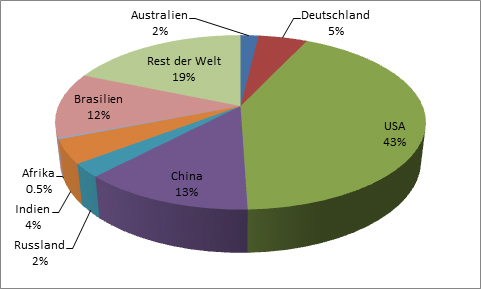
\includegraphics[width=0.8\textwidth]{images/global_revenue_share.jpg} 
  \caption{Anteile am IT-Consulting Weltmarkt} \label{fig:weltmarkt} 
\end{figure}


\item {Deutschland}

Das Wachstum des deutschen IT-Consulting ist mit 8,4\% sehr hoch im Verhältnis des Wirtschaftswachstums von 3\% in 2011.\cite{statGer2} Dabei haben die Top 25 IT-Consulting Unternehmen sogar noch ein größeres Wachstum mit Spitzen bis zu 10\%. \cite[6]{topITB} Dies sind durchaus überdurchschnittliche Wachstumsraten, welche international mit aufsteigenden Ökonomien wie Indien, Russland oder China sehr gut mithalten können. Der Gesamtumsatz des IT-Consulting beträgt 29,4 Milliarden Euro.  Das sind 1,12 Prozent des gesamten bereinigten Bruttoinlandproduktes. \cite{statGer} Um die Dichte des IT-Consultingmarktes einschätzen zu können macht es Sinn den Gesamtumsatz auf die Ländergröße zu beziehen. 
Deutschland schneidet hier mit 8,24 Milliarden Euro pro 100000 km² ab. Dies ist im Verhältnis mit anderen Ländern eine recht hohe Dichte und bietet daher Wegersparnisse und Kommunikationsvorteile die sich strategisch günstig auswirken können.

\item {USA}

Die USA zweifellos einen gigantischen Marktanteil an IT-Services. Mit 244 Milliarden Euro, was 43\% des weltweiten IT-Service Markt einnimmt, ist es mit Abstand das umsatzstärkste Land der Welt im Bereich IT-Services. \cite{ibisUSA} Das Wachstum stagniert allerdings mit 2,2\%. Im Verhältnis zum Wachstum des bereinigten Bruttoninlandprodukt von 1,8\% wächst es nur wenig mehr. \cite{statUSA} Die Umsatzdichte beträgt 2,48 Milliarden Euro pro 100000 km². Im Verhältnis zu anderen Ländern, ist dies eine sehr hohe Dichte und schneidet damit hinter Deutschland und weit über die anderen Länder ab.
Ein Großteil der Umsätze in den USA entsteht unter anderem dadurch, dass Wertschöpfung durch IT-Services, die im Ausland durch Offshoring entstehen, hinzugerechnet werden. Diese Offshoring-Länder sind daher einer der Schlüsselfaktoren für die hohen Umsätze in den USA. (Siehe x.x)

\item {China}

China hat mit 72,6 Milliarden Euro den zweitgrößten Marktanteil der Welt. Zwar noch weniger als ein Drittel gegenüber den USA, jedoch verzeichnet es mit 6,8\% in 2011 überdurchschnittliche Wachstumsraten im Bereich IT-Services und damit hat damit das dreifache Wachstum des Konkurrenten USA.  Im Verhältnis zum  Wachstum des Bruttoinlandproduktes mit 9,2\% in 2011 ist dies jedoch verhältnismäßig wenig. Es deutet stark hier daraufhin, dass die strategische Ausrichtung der IT und deren Prozessen noch nicht  gleichermaßen Beachtung geschenkt wird, wie anderen Dienstleistungen. Mögliche Ursachen könnten Fachkräftemängel oder Kostendruck sein. Es gilt daher weiter zu untersuchen, welche Ursachen das verhältnismäßig schwache Wachstum hat. Die Dichte ist im Verhältnis zu Deutschland oder den USA auch sehr schwach. Hier schneidet China mit einer IT-Service-Dichte von 0,74 Milliarden pro 100000 km² ab. Da China sehr weitläufig und nicht vollständig industrialisiert ist, ist diese Größe wenig aussagekräftig und es besteht weiterer Untersuchungsbedarf, ob dies wirklich auf eine schwache Entwicklung hindeutet oder anderen demografischen Umständen geschuldet ist \cite{ibisChina}

\item {Russland}

Der russische Markt im Bereich IT-Services ist mit 14,3 Milliarden recht klein wenn man es auf die Größe des Landes bezieht. Es gibt vor allem viel System- und hardwarenahe Entwicklung. Dienstleistungen im IT-Sektor wachsen jedoch in zunehmenden Maße und konnten 2011 15,3\% Branchen-Wachstum erreichen. Dies ist sowohl im Vergleich zum internationalen Markt als auch im Verhältnis zum Wachstum des Bruttoinlandproduktes mit 4,3 \% in 2011 weit überdurchschnittlich. \cite{statRus2} Aufgrund der relativ kostengünstigen Entwicklungkosten für Software, insbesondere hardwarenahe Entwicklung und Systemengeneering wird Russland vor allem in Europa  zunehmend als „Offshoring Land“ attraktiv. (Wirtschaftsinformatik und Management 12/2013, Offshoring Land Russland)
Die Dichte des IT-Consulting fällt mit 84 Millionen Euro pro 100 000 km² sehr niedrig aus. Dabei ist zu berücksichtigen, dass ein Großteil von Russland gar nicht oder nur schwach bewirtschaftet ist. \cite{statRus}


\item {Afrika}

Afrika hat einen sehr niedrigen Anteil am Markt mit 1,4 Milliarden. \cite{statAfr} Statistiken zum Wachstum konnten leider nicht gefunden werden. Die großen Technologie-Beratung-Konzerne haben sich in verschiedenen Teilen Afrika als Beratungen etabliert, die auch den IT-Consulting Markt abdecken. Der Trend geht jedoch laut Experten immer mehr dahin, dass neue inländische IT-Service-Provider auf dem Markt konkurrieren und die US-Konzerne ablösen. Afrika hat 2011 mit 5\% ein durchaus gutes Wirtschaftswachstum zu verzeichnen, kann aber nicht mit anderen aufstrebenden Ökonomien mithalten, insbesondere nicht im IT-Umfeld. \cite{statAfr2}
Ursachen liegen hier nicht zuletzt in der Stromversorgung. Denn 80\% der Dörfer in Afrika sind immernoch ohne Stromversorgung, weil Energieanbietern die Vernetzung der Dörfer zu teuer ist.  \cite{dieZeit}
Die demografische Lage im gesamten Kontinent zu betrachten ist jedoch sehr vielschichtig. Eine Analyse des Marktes in sehr komplex, da dort sehr viele demografische Umbrüche stattfinden. Daher ist hier eine Betrachtung der Umsätze wenig aussagekräftig für eine klare Einschätzung. Es besteht daher hier weiterer Forschungsbedarf, um die Kennzahlen in einem differenzierteren  Kontext zu stellen.


\item {Brasilien}

Brasilien hat in 2011 mit einem Branchenumsatz von 69,6 Milliarden den drittgrößten Anteil am IT-Consulting Markt. Das Wachstum über die Jahre von 2008-2011 beträgt 61\%. \cite{statBras2} Trotz seiner flächenmäßigen Größe weist es dadurch mit 0,82 Milliarden pro 100 000 km eine verhältnismäßig hohe Dichte auf. Das Wachstum in 2011 in der IT-Services-Branche beträgt hier 4,9\% und ist damit weitaus höher als das Gesamtwirtschaftswachstum mit 2,7\%. Dabei beträgt der Anteil am Bruttoinlandprodukt allein 4,5\%. Dies zeigt welchen großen Stellenwert der Markt für IT-Services in Brasilien einnimmt. Experten prognostizieren weiterhin einen rasanten Anstieg des Wachstums, insbesondere im Bereich BPO, welche laut Schätzungen 85\% am Gesamtmarktanteil einnimmt.\cite{statBras}

\item {Zusammenfassung}

Alle Werte beziehen sich auf die Jahre von 2011 bis 2012. Die entsprechenden Quellen sind in den Länderabschnitten zu finden.



\begin{tabular}{|p{2.6cm}|p{1.5cm}|p{2cm}|p{1.5cm}|p{1.5cm}|p{1.7cm}|}
 \hline
  \textbf{Land} & \textbf{Umsatz in Mrd. €} & \textbf{IT-Consulting Wachstum} & \textbf{BIP Wachstum} & \textbf{Welt-Markt-Anteil} & \textbf{Umsatz-Dichte in Mrd. € pro 100 000 km²} \\
  \hline
    
    1. USA  & 244,33  &2,2\%  & 1,8\% & 43\% & 2,48  \\
    2. China & 72,50 & 6,8\%  & 9,2\% & 13\% & 0,74 \\
    3. Brasilien & 69,60 & 4,9\%  & 2,7\% & 12\% & 0,817 \\
    4. Deutschland & 29,4 & 8,5\%  & 3\% & 5\% & 8,24 \\
    5. Indien & 25,45  & 11.2\%  & 7.9\% & 4\% & 0,77  \\
    6. Russland & 14,3  & 15.4\%  & 4,3\% & 2\% & 0,084  \\
    7. Afrika & 1.4  & n/a  & 5\% & 0.5\% & 0,0046 \\
 \hline
\end{tabular}


\end{itemize}


